\documentclass[]{auvsi_doc}
\setkeys{auvsi_doc.cls}{
	AUVSITitle={Unmanned Ground Vehicle (UGV) Parachute Testing Description}
	%AUVSILogoPath={./logo.pdf]}
}

% include extra packages, if needed
\usepackage{longtable}
\usepackage{gensymb}
\usepackage{subcaption}


\begin{document}

\begin{AUVSITitlePage}
\begin{artifacttable}
\entry{GV-003, 0.1, 2018-10-30, Initial Draft, John Akagi, Kameron Eves}
\entry{GV-003, 1.0, 2018-11-6, Revised after design review, John Akagi, Andrew Torgesen}
\entry{GV-003, 1.1, 2018-11-8, Added Intro and Conclusion. Fixed minor errors, Brady Moon, John Akagi and Tyler Critchfield}
% additional \entry{} commands for extra rows in the revision table, if needed
\end{artifacttable}
\end{AUVSITitlePage}

\section{Introduction}
This artifact details the methods and results of testing parachute UGV drop system concepts from GV-001.

\section{Parachute Testing}
The parachute concepts were tested in the high bay in the Engineering Research Lab. There is scaffolding that allowed us an approximately 35~foot drop into a 20~foot by 10~foot area. Initial testing was done on the methods to measure the landing velocity of the payload and to get a basic understanding of what variables were important to control. After the initial testing, we decided to test a large parachute, a small parachute, and a small parachute with control fins on the payload because these seemed to have the largest impact on the precision of the drop and the landing speed. The large parachute was 48~inches in diameter with a 16~inch diameter spill hole. The small parachute was 30~inches in diameter with a 6~inch diameter spill hole. The fin design was comprised of two fins with a total surface area of 19.5~in\textsuperscript{2}.

We tested these three methods by dropping each one three times and recording the impact point to evaluate how well the drop system met the key success measure of airdrop accuracy. The payload weight for each drop was .711~kg.  During these drops, we controlled the position, shape, and orientation of the parachute to reduce any effects that would be caused by imperfections in the construction of our parachute. For the drop with the fins, the fins were both oriented at approximately a 45\degree angle relative to vertical and turned to the right to try and offset the leftward drift of the small parachute. The parachute and setup for the parachute connections are shown in Figure \ref{fig:combined}. The results of the test are shown in Table \ref{table:results} and the drop locations are shown in Figure \ref{fig:locations}.

For each drop, the parachute was held on two opposite side in a way to try and equalize the tension in each of the parachute cords. The payload was allowed to hang freely beneath the parachute, although the parachute was not released until any twisting motion of the payload had been damped out. Each payload was released from approximately the same place which was determined by visually lining the payload up with a target placed on the ground. The parachute was released into still air and the position of the initial impact was recorded by an observer on the ground. If the payload impacted the wall before reaching the ground, the observer would extrapolate the ground impact location by estimating the lateral speed and height of impact. The average initial impact position and the standard deviation of the spread were calculated. 

Since we could only drop from a height of about 35~ft, the average impact position and standard deviation were calculated for a 100~ft drop using a simple linear extrapolation. We assumed that the payload would drift approximately 3 times as far in a 100~ft drop as it would in a 35~ft drop,  multiplied the landing distances by that factor, and recalculated the standard deviation. While the actual payload drop will likely be less accurate due to cross winds and being dropped with an initial lateral velocity, these tests are useful in determining the relative accuracy of various delivery systems in ideal conditions. Additionally, based on our observations during the tests, we concluded that the parachutes were fully inflated and were at or close to terminal velocity when they reached the ground. 

The landing speed was estimated by filming the impact of the payload and comparing the change in position of the payload between frames to a known measurement that was visible in the camera frame. The estimated velocities are reported in Table \ref{table:results_v}. As stated before, our subjective observations lead us to believe that the payloads were at terminal velocity when they hit the ground and so there will be little change in impact velocity between these tests and dropping the payloads from 100 ft. Although the smaller parachute has a velocity about twice the velocity of the large parachute, we did not feel that any of these hits would cause the destruction of the water bottle or UGV. Additionally, we feel that the appropriate addition of shock absorbers, crumple zones, padding, or other dampers would further increase the survivability of the UGV.

\begin{table}[h!]
\caption{The results of dropping the three different parachute systems. The average distance is the average lateral distance between the dropping and landing positions. The standard deviation is the standard deviation between all three drops for each system. The scaled standard deviation is the estimated standard deviation when payloads are dropped from 100~ft. }
\label{table:results}

\begin{tabular}{| l | l | l | l |}
\hline
Method & Average Distance & Std. Deviation & Scaled Std. Dev.\\
\hline
Large Parachute & 9.01~ft  & 0.95~ft & 2.85~ft\\
Small Parachute & 7.20~ft  & 1.38~ft & 4.14~ft\\
Small Parachute with Fins & 4.70~ft & 1.08~ft & 3.23~ft\\
\hline

\end{tabular}

\end{table}

\begin{table}[h!]
\caption{Estimated landing velocities of the parachute concepts. Landing speeds were calculated by filming the impact and comparing the change of position in the bottle between frames. These distances were then compared to a known measurement that was also in the video frame.}
\label{table:results_v}

\begin{tabular}{| l | l |}
\hline
Method & Impact Velocity\\
\hline
Large Parachute & 2.7~m/s \\
Small Parachute & 4.8~m/s \\
Small Parachute with Fins & 4.8~m/s \\
\hline

\end{tabular}

\end{table}

\section{Glider Testing}
A rough prototype was constructed based on a simple glider design in XFLR5 that was designed to carry a payload of 1~kg (see Figure X). The prototype had a span of about 1~m and a mean aerodynamic center of 10~cm. In testing we taped a small water bottle to the underside of the glider and dropped it from heights of 5~ft, 6~ft, and 7~ft (10 times for each height). The location it hit the ground was recorded and a standard deviation was calculated that was then extrapolated to a height of 100~ft. These results are summarized in the artifact GV-004 UGV Drop Mechanism Concept Test Procedures and Results. One takeaway we learned was that our prototype could not support the designed weight. We assume this is because we were not testing it at its design velocity, and understand that this test was not very realistic. However, it did have adequate consistency with a small payload. This proves that with more design and better test procedures, the glider could perform well. 

\begin{figure}[h!]
	\centering
	\begin{subfigure}{0.49\linewidth} \centering
		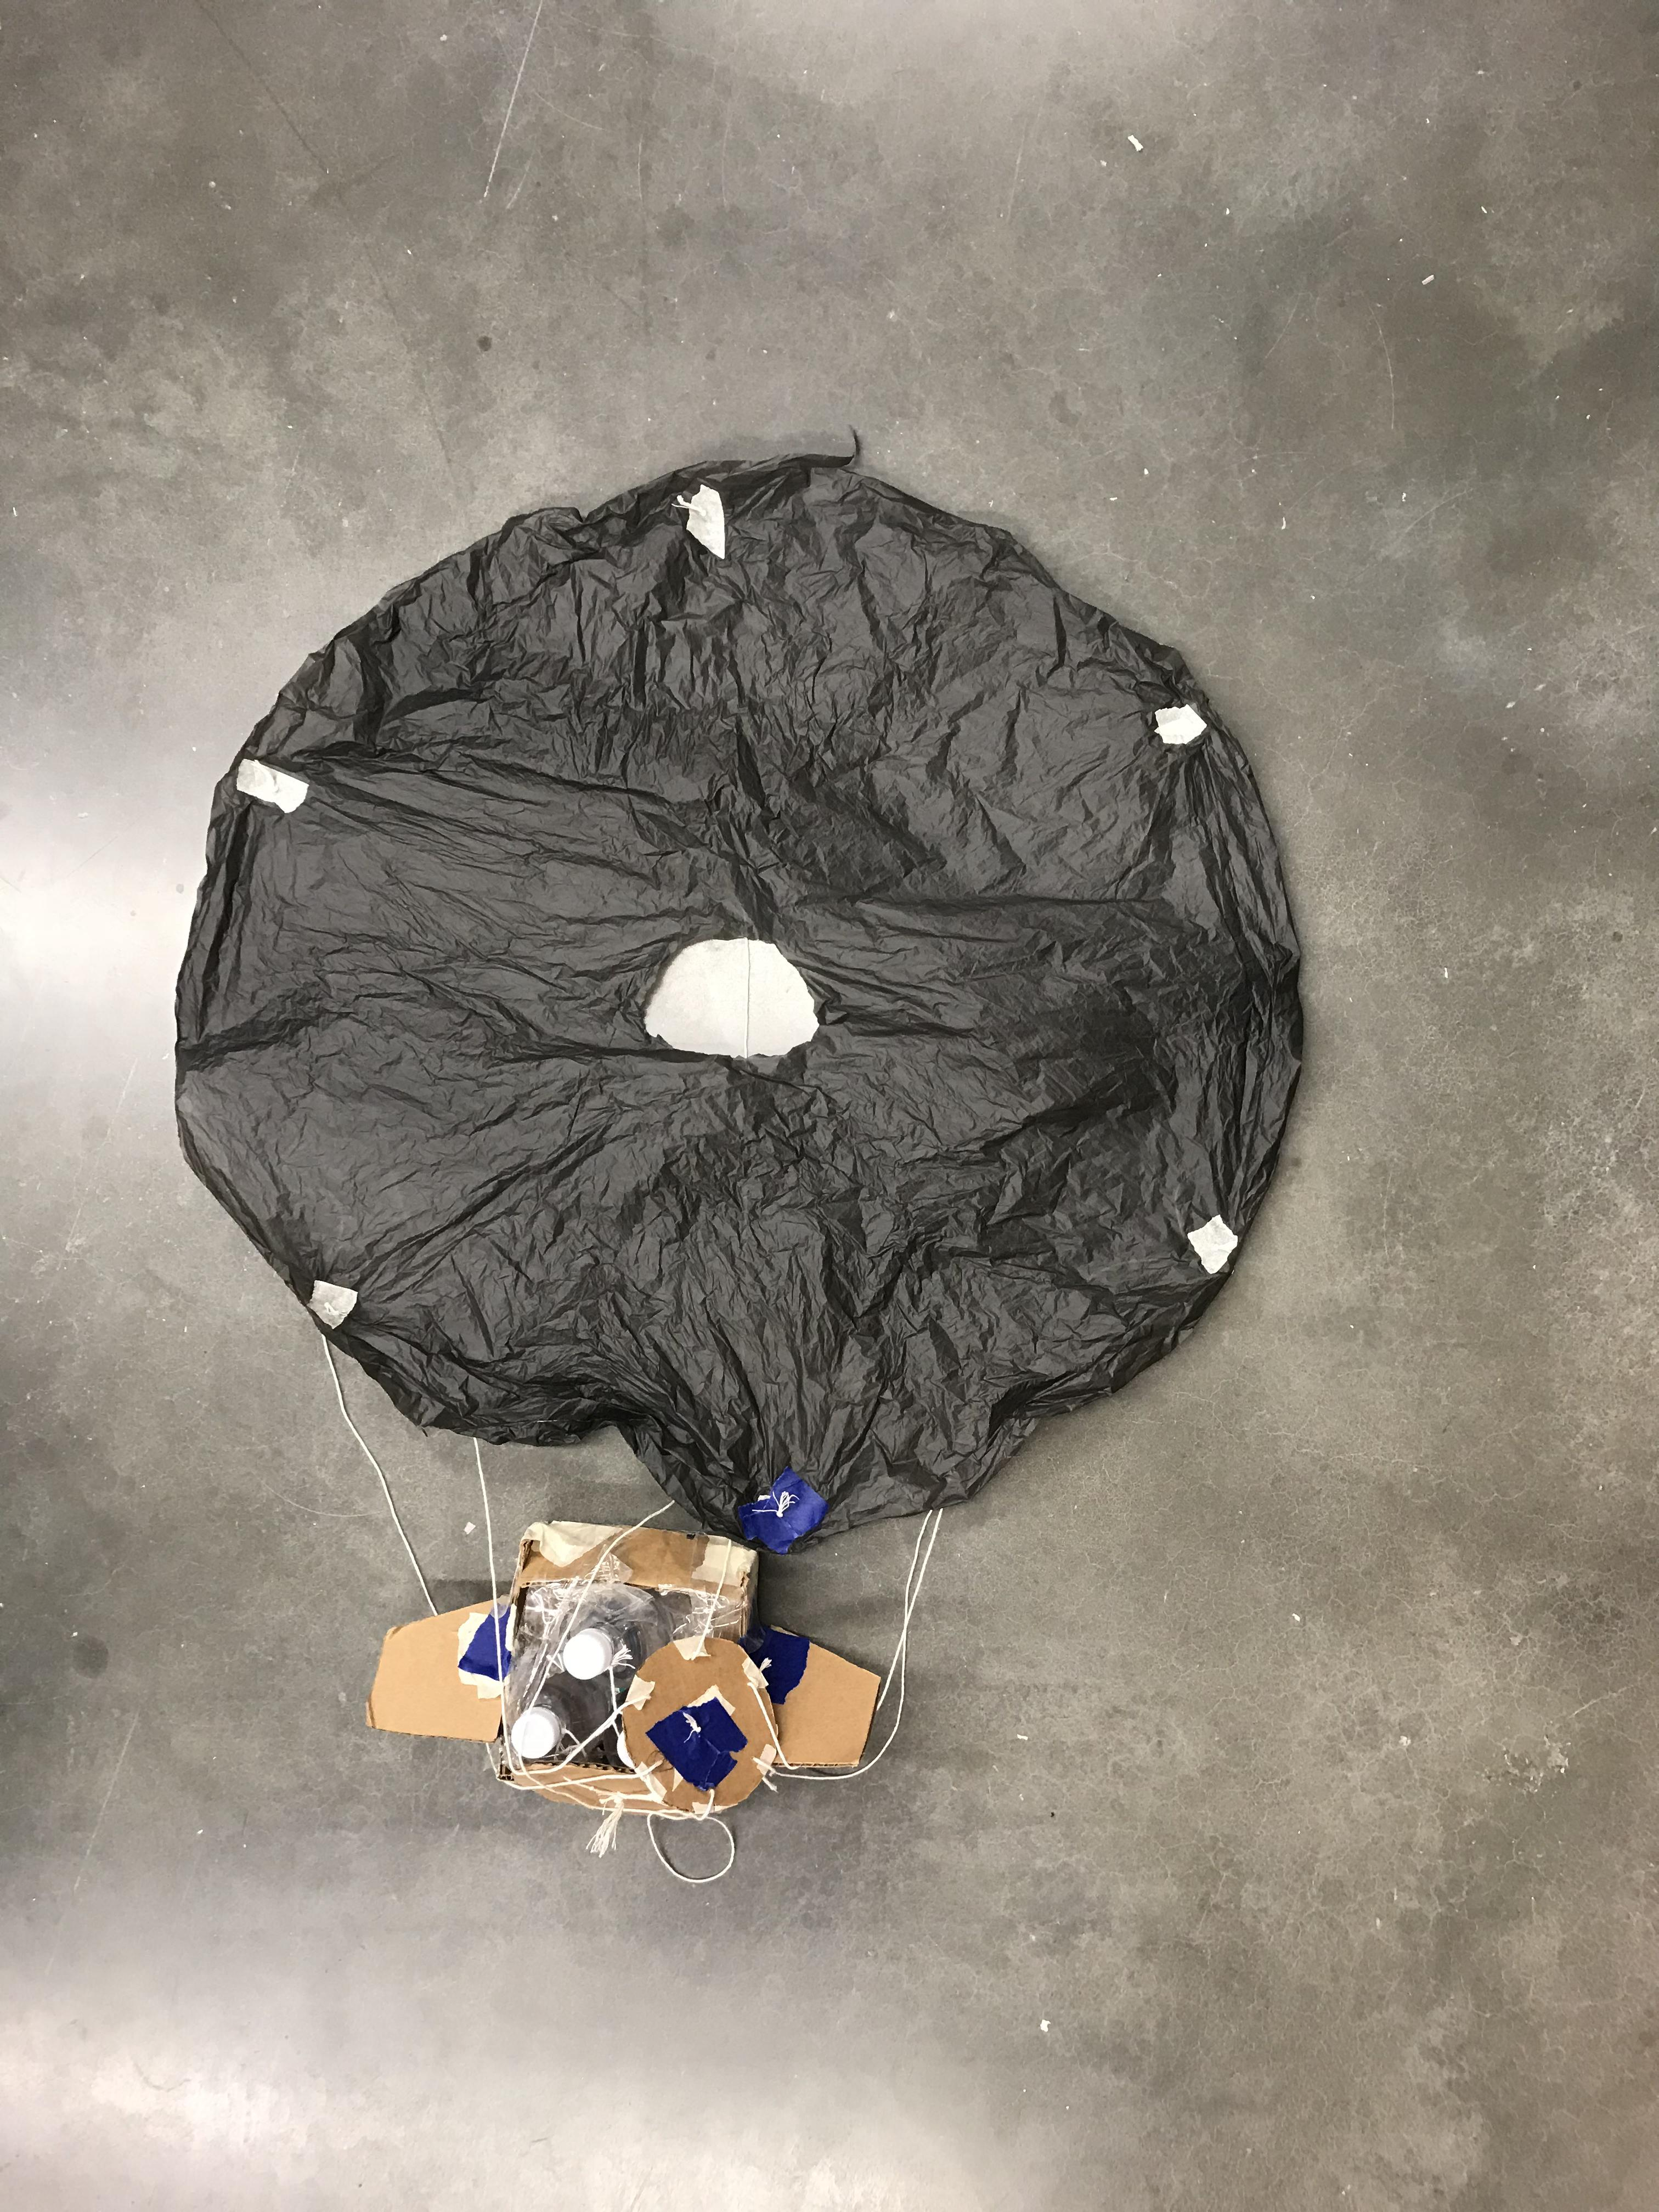
\includegraphics[width=.95\columnwidth]{Parachute1.jpg}
		\caption{Full configuration for parachute and fins.}\label{fig:fullParachute}
	\end{subfigure}
	\begin{subfigure}{0.49\linewidth} \centering
		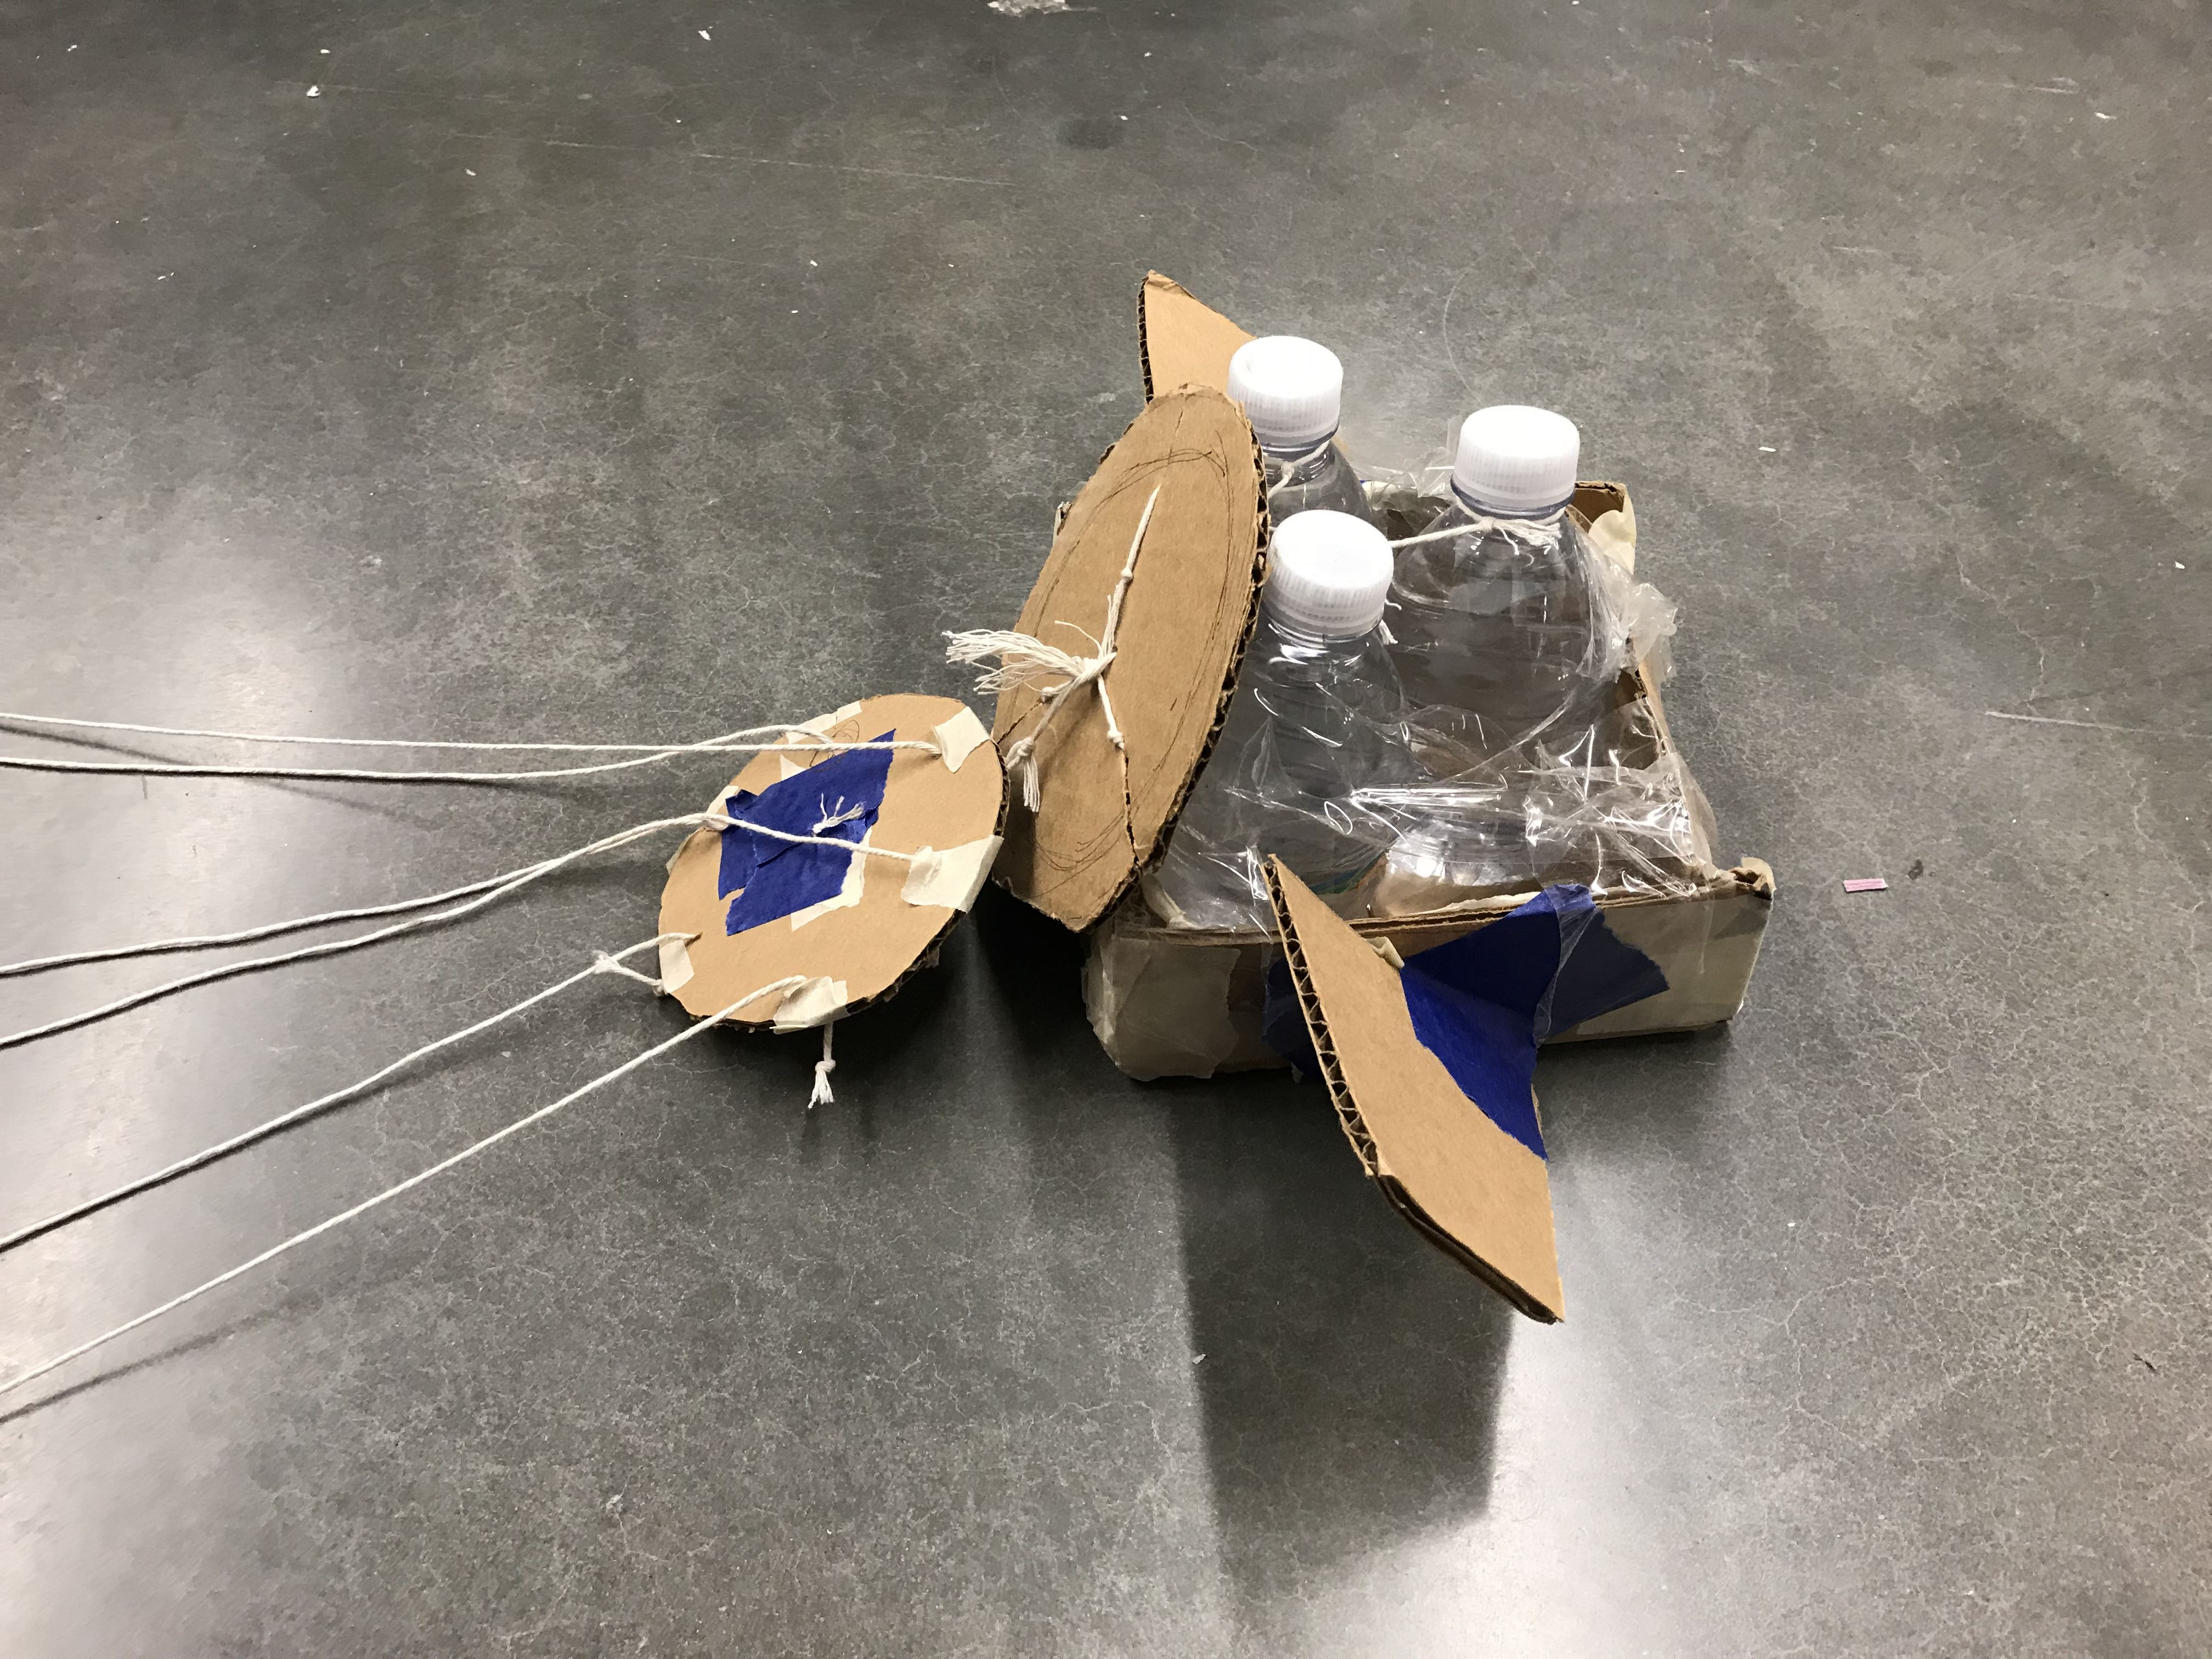
\includegraphics[width=.95\columnwidth]{Parachute2.jpg}
		\caption{Control fins and connections to parachute.}\label{fig:ControlFins}
	\end{subfigure}
	\caption{Testing setup for the small parachute and fins option. The small parachute only method was the same but without the cardboard holder around the water bottles. The large parachute method was identical to the small parachute method but simply larger.}
	\label{fig:combined}
\end{figure}


\begin{figure}[h!]
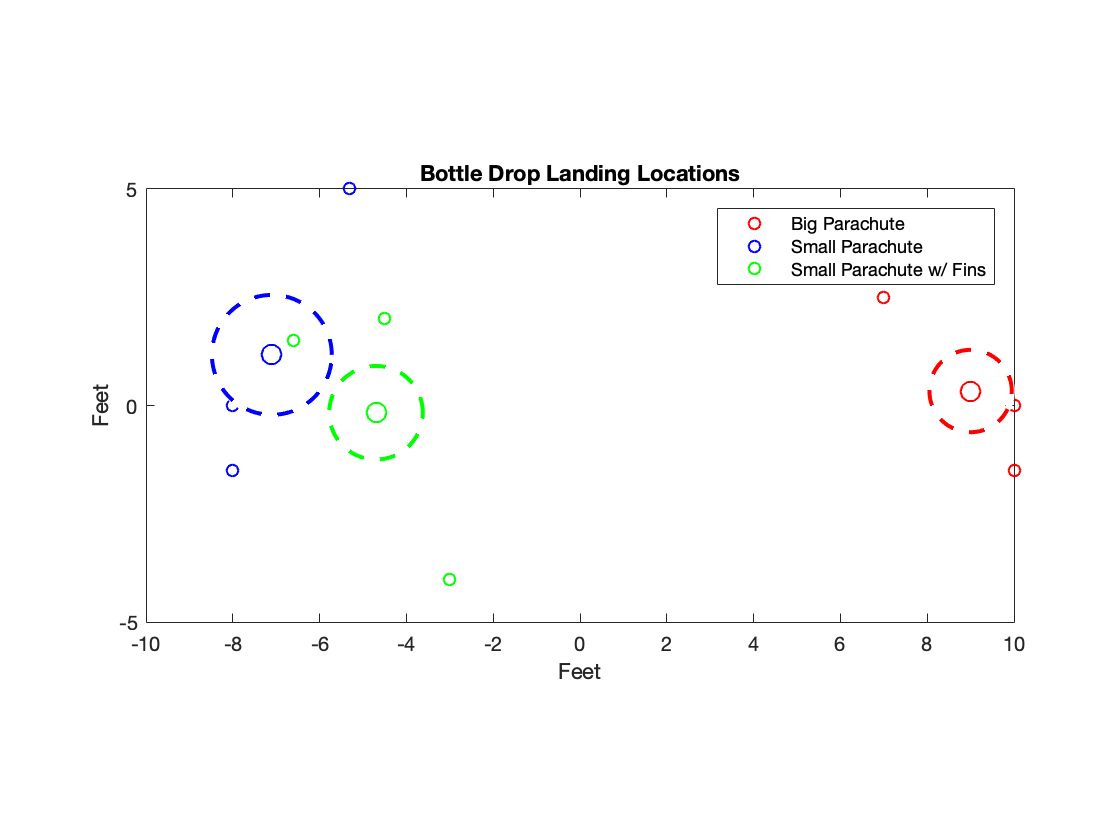
\includegraphics[width=\columnwidth]{LandingLocations.png}
\caption{The location of the initial impacts of each of the drops as shown by filled in circles. Due to the constrained area of our testing location, some landing locations were extrapolated since they hit the walls before the ground. The open circles are the average location of impact. The dashed lines indicate the mean distance away from the average impact location. The colors differentiate between system types as shown in the legend.}
\label{fig:locations}
\end{figure}

\begin{figure}[h!]
	\centering
	\begin{subfigure}{0.49\linewidth} \centering
		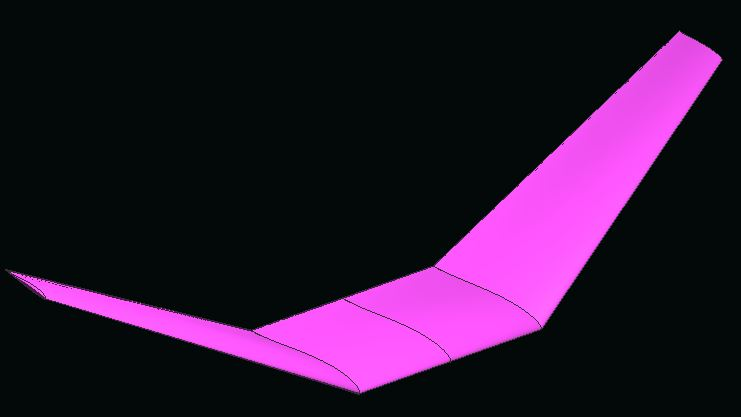
\includegraphics[width=.95\columnwidth]{glider1.jpg}
		\caption{Simple prototype model simulated in XFLR5.}
		\label{fig:glidermodel}
	\end{subfigure}
	\begin{subfigure}{0.49\linewidth} \centering
		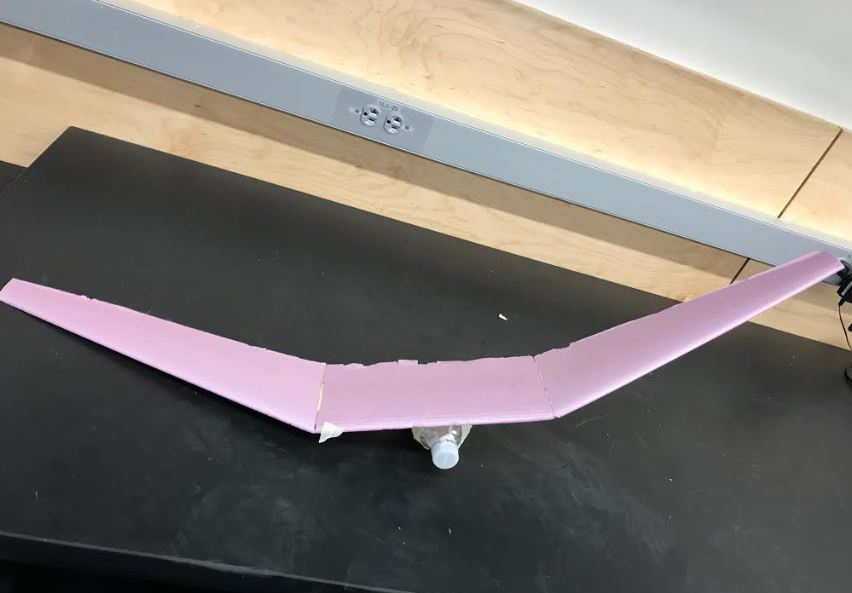
\includegraphics[width=.95\columnwidth]{glider2.jpg}
		\caption{Constructed glider prototype.}
		\label{fig:glider}
	\end{subfigure}
	\caption{Testing setup for the glider concept. A simple model was built in XFLR5. This was then built by using the foam cutter to cut out each of the 3 sections. These sections were glued together with a spar in the middle section. A water bottle payload was taped underneath.}
	\label{fig:combined}
\end{figure}

\newpage

\section{Conclusion}
Parachute drop concepts were tested in the Engineering Research Lab high bay for landing velocity and precision. Test results are used in artifact GV-004 for overall comparison of our concepts.




\end{document}
